\subsection{File Transfer: FTP}

\begin{figure}[h]
\centering
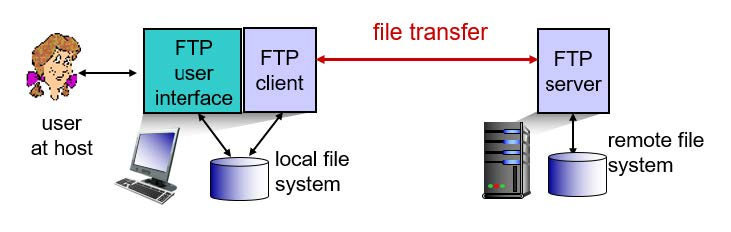
\includegraphics[width=4.5in]{./img/imghfdst2/ftp.jpg}
\caption{Voorbeeld van een ftp }
\label{fig:ftp}
\end{figure}

\noindent \textbf{functie}: bestanden overbrengen naar en van een remote host.

Client/server model:
\bi
\itf Client: de kant dat de overdracht start (eender in welke richting).
\itf Server: de remote host
\ei

ftp: RFC 959

ftp server: port 21

FTP maakt gebruik van 2 parallelle TCP-verbindingen voor het overbrengen van een bestand. De \textbf{besturingsverbinding} en de \textbf{gegevensverbinding}.

\textbf{Besturingsverbinding}: Wordt gebruikt om controle-informatie tussen de twee hosts uit te wisselen (gebruikersnaam, wachtwoord, PUT, GET, ...).

\textbf{Gegevensverbinding}: Wordt gebruikt voor het verzenden van het eigenlijke bestand. Het bestand wordt op een andere verbinding verzonden als de controle-informatie en wordt dus out-of-band genoemd.
Gang van zaken

\be
\itf Client legt TCP-besturingsverbinding aan met een server.
\itf Client stuurt gebruikersnaam en wachtwoord via de besturingsverbinding. (Alsook de mappen/bestanden die geselecteerd worden)
\itf Wanneer de server het bevel krijgt om een bestand door te sturen legt de server een gegevensverbinding aan met de client.
\itf Er wordt 1 bestand verstuurd door de gegevensverbinding en wordt vervolgens verbroken. Voor elk nieuw bestand dat moet worden verzonden, wordt een nieuwe verbinding gemaakt.
\itf (FTP houdt de status van de client in de gaten om te zien tot welke mappen hij allemaal toegang heeft)
\ee

\subsubsection{FTP commando’s en antwoorden}

De commando’s van de client naar server, en antwoorden van server naar client zijn verzonden door de controle connectie in een 7 bit ASCII formaat. Dus dit is ook leesbaar voor mensen. Elk commando bestaat uit vier hoofdletter ASCII tekens, sommige met extra argumenten. Sommige van de meest gebruikte commando’s:
\begin{itemize}
   \item USER username: gebruikt om de gebruikers identificatie naar de server te sturen
\item PASS password: gebruikt om het wachtwoord naar de server te sturen
\item LIST: een lijst van alle files terug te sturen van de huidige remote directory.
\item RETR filename: gebruikt om een bestand van de huidige directory van de remote host op te halen.
\item STOR filename: gebruikt om een bestand in de huidige directory van de remote host te stoppen.
\end{itemize}

